%!TEX root = ../main/main.tex
\section{Architectural styles and patterns} % (fold)
\label{sec:architectural_styles_and_patterns_}
This section highlights both hardware and software selected styles and design patterns.\\
It's important to underline that the rules described below are just a general guideline for the actual developers of the project.\\
During the development phase it's often required to switch style or rely on other patterns to carry on.\\
Developers should not recur to \emph{hacks} in order to comply with design rules provided while the \emph{system to be} is not fully specified.
\subsection{Software styles and patterns} % (fold)
\label{sub:software_styles_and_patterns}
The overall software system must follow the \emph{Object Oriented Paradigm}.\\
In particular, developers should follow the principles of \emph{encapsulation}, \emph{composition}, \emph{inheritance}, \emph{delegation} and \emph{polymorphism}.\\
Developers should promote code reuse and should try to solve programming problems using common \emph{OO Design Patterns}\footnote{\emph{See Design Patterns:
Elements of Reusable Object-Oriented Software} by Erich Gamma,
Richard Helm,
Ralph Johnson,
John Vlissides}.\\
Code produced by develpers, must be fully commented and documented in order to promote simple refactoring and maintenance.
\subsection{Harwdare styles and patterns} % (fold)
\label{sub:harwdare_styles_and_patterns}
As outlined in \emph{section \ref{sec:deployment_view}}, our hardware system is based on a \emph{2 tier} architecture:
\begin{itemize}
	\item \textbf{First Tier} The first tier is composed of \emph{clients} devices. Such as mobile phone, tablets, and browser enabled computers.
	\item \textbf{Second Tier} The second tier is composed of a rack of \emph{Servers} controlled by a load balancing component.
\end{itemize}
From the logical point of view, our system is divided in \emph{3 layers}:
\begin{itemize}
	\item \textbf{Presentation Layer} This layer is responsible for displaying data to the users and for transmitting input data to the \emph{business logic layer}. The \emph{presentation layer} is deployed in the \emph{First Tier}.
	\item \textbf{Business Logic Layer} This layer is responsible for receiving data from the \emph{presentation layer}, for computing and transmitting a response (using also data provided by the \emph{data store layer}) to the presentation layer.\\
	This layer implements most of the business logic and is deployed in the \emph{second tier}.
	\item \textbf{Data Store Layer} This layer is responsible for storing all the data meaningful to the system. This layer is deployed in the \emph{second tier}.
\end{itemize}
A schema of the overall architecture is provided below.
\begin{figure}[h!t]
\caption{Architecture Diagram}
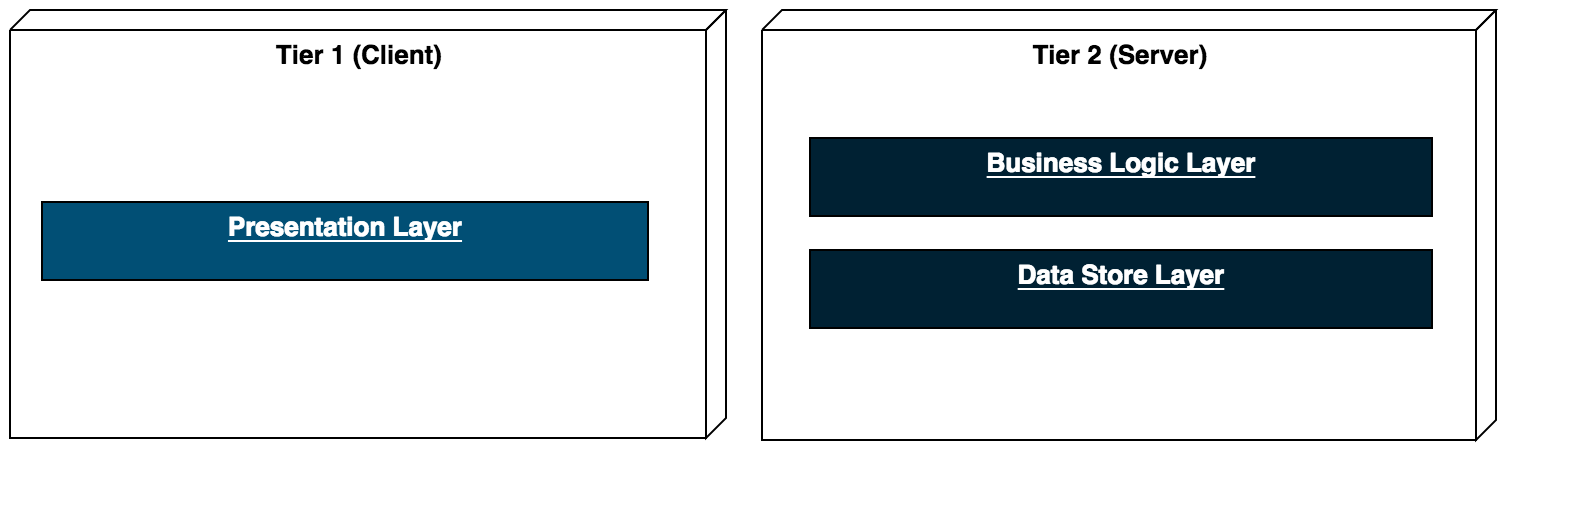
\includegraphics[width=\textwidth]{diagram/png/architecture}
\centering
\end{figure}
\newpage



% subsection software_styles_and_patterns (end)

% subsection harwdare_styles_and_patterns (end)
% section architectural_styles_and_patterns_ (end)